\documentclass[11pt]{article}
\usepackage[preprint]{acl}
\geometry{letterpaper,margin=1in}
\usepackage{times}
\usepackage{latexsym}
\usepackage[T1]{fontenc}
\usepackage[utf8]{inputenc}
\usepackage[protrusion=false]{microtype}
\usepackage{graphicx}
\usepackage{booktabs}
\usepackage{amsmath}
\usepackage{xcolor}
\newcommand{\MedianRaters}{4}
\newcommand{\BorderlineShare}{18\%}
\newcommand{\LeakTrain}{404}
\newcommand{\LeakVal}{44}
\newcommand{\LeakTest}{123}
\newcommand{\NTrain}{267,112}
\newcommand{\NVal}{45,003}
\newcommand{\NTest}{132,607}
\newcommand{\Best}{\texttt{bert\_distil\_soft}}
\newcommand{\IGTopErm}{13\%}
\newcommand{\IGTopBest}{27\%}
\newcommand{\IGTopThreeErm}{56\%}
\newcommand{\IGTopThreeBest}{64\%}
\newcommand{\FPFixed}{945}
\newcommand{\FPIntro}{1,494}
\newcommand{\FPErm}{6,666}
\newcommand{\FPBest}{7,215}
\newcommand{\FNFixed}{687}
\newcommand{\FNIntro}{369}
\newcommand{\FNErm}{4,399}
\newcommand{\FNBest}{4,081}
\newcommand{\HandFPIdentity}{28}
\newcommand{\HandFPCivil}{27}
\newcommand{\HandFNCivil}{24}
\newcommand{\HandFNImplicit}{30}
\newcommand{\HandFNSarcasm}{13}
\newcommand{\HandOther}{5}
\newcommand{\HandGoldWrong}{23}
\newcommand{\HandAmbiguous}{18}
\newcommand{\HandIdTagFP}{59 of 100}
\newcommand{\HandQuoteTag}{14 of 17}
\newcommand{\HandQuoteTagElse}{45 of 183}
\newcommand{\HandSarcTag}{2 of 20}
\newcommand{\TokMedian}{60}
\newcommand{\TokOverOneTwoEight}{21\%}
\newcommand{\TokOverTwoFiveSix}{0.2\%}
\newcommand{\TokToxicOverOneTwoEight}{18\%}
\newcommand{\ToxicShare}{11\%}
\newcommand{\BenignIdRater}{45\%}
\newcommand{\BenignNoIdRater}{24\%}
\newcommand{\BenignIdFrac}{0.112}
\newcommand{\BenignNoIdFrac}{0.054}
\newcommand{\SmallestGroupN}{988}
\newcommand{\MajorityAuc}{0.500}
\newcommand{\MajorityFOne}{0.000}
\newcommand{\MajorityAcc}{0.886}
\newcommand{\MajorityBiasAuc}{0.500}
\newcommand{\MajorityWorstGroupAcc}{0.000}
\newcommand{\MajorityMeanAbsFprGap}{0.000}
\newcommand{\MajorityMaxFprGap}{0.000}
\newcommand{\MajorityEceRaw}{0.114}
\newcommand{\MajorityEceCal}{0.114}
\newcommand{\MajorityThreshold}{0.500}
\newcommand{\MajorityTemperature}{1.000}
\newcommand{\TfidfErmAuc}{0.912}
\newcommand{\TfidfErmFOne}{0.599}
\newcommand{\TfidfErmAcc}{0.909}
\newcommand{\TfidfErmBiasAuc}{0.871}
\newcommand{\TfidfErmWorstGroupAcc}{0.509}
\newcommand{\TfidfErmMeanAbsFprGap}{0.103}
\newcommand{\TfidfErmMaxFprGap}{0.231}
\newcommand{\TfidfErmEceRaw}{0.015}
\newcommand{\TfidfErmEceCal}{0.015}
\newcommand{\TfidfErmCfTemplateGap}{0.133}
\newcommand{\TfidfErmCfTemplateGapSeen}{0.148}
\newcommand{\TfidfErmCfTemplateGapHeldout}{0.020}
\newcommand{\TfidfErmCfRealDelta}{0.041}
\newcommand{\TfidfErmTemplateNeutralFlagRate}{0.201}
\newcommand{\TfidfErmAurc}{0.023}
\newcommand{\TfidfErmErrAtEightycov}{0.037}
\newcommand{\TfidfErmThreshold}{0.260}
\newcommand{\TfidfErmTemperature}{0.993}
\newcommand{\TfidfErmeightyAuc}{0.894}
\newcommand{\TfidfErmeightyFOne}{0.569}
\newcommand{\TfidfErmeightyAcc}{0.897}
\newcommand{\TfidfErmeightyBiasAuc}{0.847}
\newcommand{\TfidfErmeightyWorstGroupAcc}{0.478}
\newcommand{\TfidfErmeightyMeanAbsFprGap}{0.124}
\newcommand{\TfidfErmeightyMaxFprGap}{0.277}
\newcommand{\TfidfErmeightyEceRaw}{0.025}
\newcommand{\TfidfErmeightyEceCal}{0.024}
\newcommand{\TfidfErmeightyCfTemplateGap}{0.101}
\newcommand{\TfidfErmeightyCfTemplateGapSeen}{0.114}
\newcommand{\TfidfErmeightyCfTemplateGapHeldout}{0.029}
\newcommand{\TfidfErmeightyCfRealDelta}{0.037}
\newcommand{\TfidfErmeightyTemplateNeutralFlagRate}{0.194}
\newcommand{\TfidfErmeightyAurc}{0.029}
\newcommand{\TfidfErmeightyErrAtEightycov}{0.048}
\newcommand{\TfidfErmeightyThreshold}{0.200}
\newcommand{\TfidfErmeightyTemperature}{0.952}
\newcommand{\TfidfReweightAuc}{0.884}
\newcommand{\TfidfReweightFOne}{0.568}
\newcommand{\TfidfReweightAcc}{0.903}
\newcommand{\TfidfReweightBiasAuc}{0.856}
\newcommand{\TfidfReweightWorstGroupAcc}{0.432}
\newcommand{\TfidfReweightMeanAbsFprGap}{0.038}
\newcommand{\TfidfReweightMaxFprGap}{0.089}
\newcommand{\TfidfReweightEceRaw}{0.108}
\newcommand{\TfidfReweightEceCal}{0.089}
\newcommand{\TfidfReweightCfTemplateGap}{0.155}
\newcommand{\TfidfReweightCfTemplateGapSeen}{0.173}
\newcommand{\TfidfReweightCfTemplateGapHeldout}{0.080}
\newcommand{\TfidfReweightCfRealDelta}{0.047}
\newcommand{\TfidfReweightTemplateNeutralFlagRate}{0.125}
\newcommand{\TfidfReweightAurc}{0.028}
\newcommand{\TfidfReweightErrAtEightycov}{0.045}
\newcommand{\TfidfReweightThreshold}{0.630}
\newcommand{\TfidfReweightTemperature}{0.829}
\newcommand{\TfidfCdaAuc}{0.906}
\newcommand{\TfidfCdaFOne}{0.591}
\newcommand{\TfidfCdaAcc}{0.906}
\newcommand{\TfidfCdaBiasAuc}{0.867}
\newcommand{\TfidfCdaWorstGroupAcc}{0.509}
\newcommand{\TfidfCdaMeanAbsFprGap}{0.092}
\newcommand{\TfidfCdaMaxFprGap}{0.199}
\newcommand{\TfidfCdaEceRaw}{0.011}
\newcommand{\TfidfCdaEceCal}{0.011}
\newcommand{\TfidfCdaCfTemplateGap}{0.135}
\newcommand{\TfidfCdaCfTemplateGapSeen}{0.109}
\newcommand{\TfidfCdaCfTemplateGapHeldout}{0.031}
\newcommand{\TfidfCdaCfRealDelta}{0.011}
\newcommand{\TfidfCdaTemplateNeutralFlagRate}{0.271}
\newcommand{\TfidfCdaAurc}{0.024}
\newcommand{\TfidfCdaErrAtEightycov}{0.040}
\newcommand{\TfidfCdaThreshold}{0.270}
\newcommand{\TfidfCdaTemperature}{1.035}
\newcommand{\TfidfSoftAuc}{0.914}
\newcommand{\TfidfSoftFOne}{0.593}
\newcommand{\TfidfSoftAcc}{0.901}
\newcommand{\TfidfSoftBiasAuc}{0.866}
\newcommand{\TfidfSoftWorstGroupAcc}{0.604}
\newcommand{\TfidfSoftMeanAbsFprGap}{0.143}
\newcommand{\TfidfSoftMaxFprGap}{0.282}
\newcommand{\TfidfSoftEceRaw}{0.046}
\newcommand{\TfidfSoftEceCal}{0.027}
\newcommand{\TfidfSoftCfTemplateGap}{0.108}
\newcommand{\TfidfSoftCfTemplateGapSeen}{0.118}
\newcommand{\TfidfSoftCfTemplateGapHeldout}{0.026}
\newcommand{\TfidfSoftCfRealDelta}{0.036}
\newcommand{\TfidfSoftTemplateNeutralFlagRate}{0.146}
\newcommand{\TfidfSoftAurc}{0.024}
\newcommand{\TfidfSoftErrAtEightycov}{0.042}
\newcommand{\TfidfSoftThreshold}{0.200}
\newcommand{\TfidfSoftTemperature}{0.721}
\newcommand{\TfidfComboAuc}{0.889}
\newcommand{\TfidfComboFOne}{0.562}
\newcommand{\TfidfComboAcc}{0.897}
\newcommand{\TfidfComboBiasAuc}{0.854}
\newcommand{\TfidfComboWorstGroupAcc}{0.474}
\newcommand{\TfidfComboMeanAbsFprGap}{0.070}
\newcommand{\TfidfComboMaxFprGap}{0.163}
\newcommand{\TfidfComboEceRaw}{0.091}
\newcommand{\TfidfComboEceCal}{0.005}
\newcommand{\TfidfComboCfTemplateGap}{0.108}
\newcommand{\TfidfComboCfTemplateGapSeen}{0.094}
\newcommand{\TfidfComboCfTemplateGapHeldout}{0.041}
\newcommand{\TfidfComboCfRealDelta}{0.009}
\newcommand{\TfidfComboTemplateNeutralFlagRate}{0.188}
\newcommand{\TfidfComboAurc}{0.028}
\newcommand{\TfidfComboErrAtEightycov}{0.047}
\newcommand{\TfidfComboThreshold}{0.280}
\newcommand{\TfidfComboTemperature}{0.538}
\newcommand{\BertErmAuc}{0.914}
\newcommand{\BertErmFOne}{0.606}
\newcommand{\BertErmAcc}{0.904}
\newcommand{\BertErmBiasAuc}{0.874}
\newcommand{\BertErmWorstGroupAcc}{0.510}
\newcommand{\BertErmMeanAbsFprGap}{0.077}
\newcommand{\BertErmMaxFprGap}{0.187}
\newcommand{\BertErmEceRaw}{0.014}
\newcommand{\BertErmEceCal}{0.007}
\newcommand{\BertErmCfTemplateGap}{0.123}
\newcommand{\BertErmCfTemplateGapSeen}{0.125}
\newcommand{\BertErmCfTemplateGapHeldout}{0.114}
\newcommand{\BertErmCfRealDelta}{0.035}
\newcommand{\BertErmTemplateNeutralFlagRate}{0.264}
\newcommand{\BertErmAurc}{0.020}
\newcommand{\BertErmErrAtEightycov}{0.038}
\newcommand{\BertErmThreshold}{0.300}
\newcommand{\BertErmTemperature}{0.888}
\newcommand{\BertCdaAuc}{0.914}
\newcommand{\BertCdaFOne}{0.605}
\newcommand{\BertCdaAcc}{0.902}
\newcommand{\BertCdaBiasAuc}{0.874}
\newcommand{\BertCdaWorstGroupAcc}{0.546}
\newcommand{\BertCdaMeanAbsFprGap}{0.094}
\newcommand{\BertCdaMaxFprGap}{0.198}
\newcommand{\BertCdaEceRaw}{0.013}
\newcommand{\BertCdaEceCal}{0.012}
\newcommand{\BertCdaCfTemplateGap}{0.088}
\newcommand{\BertCdaCfTemplateGapSeen}{0.086}
\newcommand{\BertCdaCfTemplateGapHeldout}{0.072}
\newcommand{\BertCdaCfRealDelta}{0.015}
\newcommand{\BertCdaTemplateNeutralFlagRate}{0.271}
\newcommand{\BertCdaAurc}{0.020}
\newcommand{\BertCdaErrAtEightycov}{0.036}
\newcommand{\BertCdaThreshold}{0.320}
\newcommand{\BertCdaTemperature}{0.939}
\newcommand{\BertReweightAuc}{0.896}
\newcommand{\BertReweightFOne}{0.567}
\newcommand{\BertReweightAcc}{0.892}
\newcommand{\BertReweightBiasAuc}{0.866}
\newcommand{\BertReweightWorstGroupAcc}{0.419}
\newcommand{\BertReweightMeanAbsFprGap}{0.028}
\newcommand{\BertReweightMaxFprGap}{0.051}
\newcommand{\BertReweightEceRaw}{0.189}
\newcommand{\BertReweightEceCal}{0.158}
\newcommand{\BertReweightCfTemplateGap}{0.125}
\newcommand{\BertReweightCfTemplateGapSeen}{0.135}
\newcommand{\BertReweightCfTemplateGapHeldout}{0.096}
\newcommand{\BertReweightCfRealDelta}{0.032}
\newcommand{\BertReweightTemplateNeutralFlagRate}{0.076}
\newcommand{\BertReweightAurc}{0.024}
\newcommand{\BertReweightErrAtEightycov}{0.048}
\newcommand{\BertReweightThreshold}{0.730}
\newcommand{\BertReweightTemperature}{0.752}
\newcommand{\BertDroAuc}{0.862}
\newcommand{\BertDroFOne}{0.487}
\newcommand{\BertDroAcc}{0.878}
\newcommand{\BertDroBiasAuc}{0.834}
\newcommand{\BertDroWorstGroupAcc}{0.171}
\newcommand{\BertDroMeanAbsFprGap}{0.048}
\newcommand{\BertDroMaxFprGap}{-0.041}
\newcommand{\BertDroEceRaw}{0.259}
\newcommand{\BertDroEceCal}{0.276}
\newcommand{\BertDroCfTemplateGap}{0.101}
\newcommand{\BertDroCfTemplateGapSeen}{0.101}
\newcommand{\BertDroCfTemplateGapHeldout}{0.093}
\newcommand{\BertDroCfRealDelta}{0.030}
\newcommand{\BertDroTemplateNeutralFlagRate}{0.014}
\newcommand{\BertDroAurc}{0.031}
\newcommand{\BertDroErrAtEightycov}{0.056}
\newcommand{\BertDroThreshold}{0.800}
\newcommand{\BertDroTemperature}{1.207}
\newcommand{\BertSoftAuc}{0.920}
\newcommand{\BertSoftFOne}{0.613}
\newcommand{\BertSoftAcc}{0.906}
\newcommand{\BertSoftBiasAuc}{0.880}
\newcommand{\BertSoftWorstGroupAcc}{0.567}
\newcommand{\BertSoftMeanAbsFprGap}{0.084}
\newcommand{\BertSoftMaxFprGap}{0.175}
\newcommand{\BertSoftEceRaw}{0.060}
\newcommand{\BertSoftEceCal}{0.013}
\newcommand{\BertSoftCfTemplateGap}{0.080}
\newcommand{\BertSoftCfTemplateGapSeen}{0.079}
\newcommand{\BertSoftCfTemplateGapHeldout}{0.079}
\newcommand{\BertSoftCfRealDelta}{0.027}
\newcommand{\BertSoftTemplateNeutralFlagRate}{0.146}
\newcommand{\BertSoftAurc}{0.018}
\newcommand{\BertSoftErrAtEightycov}{0.034}
\newcommand{\BertSoftThreshold}{0.260}
\newcommand{\BertSoftTemperature}{0.610}
\newcommand{\BertComboAuc}{0.914}
\newcommand{\BertComboFOne}{0.598}
\newcommand{\BertComboAcc}{0.898}
\newcommand{\BertComboBiasAuc}{0.882}
\newcommand{\BertComboWorstGroupAcc}{0.563}
\newcommand{\BertComboMeanAbsFprGap}{0.050}
\newcommand{\BertComboMaxFprGap}{0.105}
\newcommand{\BertComboEceRaw}{0.123}
\newcommand{\BertComboEceCal}{0.044}
\newcommand{\BertComboCfTemplateGap}{0.096}
\newcommand{\BertComboCfTemplateGapSeen}{0.100}
\newcommand{\BertComboCfTemplateGapHeldout}{0.073}
\newcommand{\BertComboCfRealDelta}{0.013}
\newcommand{\BertComboTemplateNeutralFlagRate}{0.111}
\newcommand{\BertComboAurc}{0.020}
\newcommand{\BertComboErrAtEightycov}{0.036}
\newcommand{\BertComboThreshold}{0.470}
\newcommand{\BertComboTemperature}{0.455}
\newcommand{\BertDistilErmAuc}{0.940}
\newcommand{\BertDistilErmFOne}{0.659}
\newcommand{\BertDistilErmAcc}{0.917}
\newcommand{\BertDistilErmBiasAuc}{0.905}
\newcommand{\BertDistilErmWorstGroupAcc}{0.614}
\newcommand{\BertDistilErmMeanAbsFprGap}{0.085}
\newcommand{\BertDistilErmMaxFprGap}{0.190}
\newcommand{\BertDistilErmEceRaw}{0.007}
\newcommand{\BertDistilErmEceCal}{0.007}
\newcommand{\BertDistilErmCfTemplateGap}{0.114}
\newcommand{\BertDistilErmCfTemplateGapSeen}{0.122}
\newcommand{\BertDistilErmCfTemplateGapHeldout}{0.088}
\newcommand{\BertDistilErmCfRealDelta}{0.038}
\newcommand{\BertDistilErmTemplateNeutralFlagRate}{0.194}
\newcommand{\BertDistilErmAurc}{0.014}
\newcommand{\BertDistilErmErrAtEightycov}{0.025}
\newcommand{\BertDistilErmThreshold}{0.330}
\newcommand{\BertDistilErmTemperature}{1.007}
\newcommand{\BertDistilCdaAuc}{0.939}
\newcommand{\BertDistilCdaFOne}{0.656}
\newcommand{\BertDistilCdaAcc}{0.918}
\newcommand{\BertDistilCdaBiasAuc}{0.904}
\newcommand{\BertDistilCdaWorstGroupAcc}{0.606}
\newcommand{\BertDistilCdaMeanAbsFprGap}{0.075}
\newcommand{\BertDistilCdaMaxFprGap}{0.156}
\newcommand{\BertDistilCdaEceRaw}{0.013}
\newcommand{\BertDistilCdaEceCal}{0.011}
\newcommand{\BertDistilCdaCfTemplateGap}{0.101}
\newcommand{\BertDistilCdaCfTemplateGapSeen}{0.094}
\newcommand{\BertDistilCdaCfTemplateGapHeldout}{0.094}
\newcommand{\BertDistilCdaCfRealDelta}{0.012}
\newcommand{\BertDistilCdaTemplateNeutralFlagRate}{0.208}
\newcommand{\BertDistilCdaAurc}{0.014}
\newcommand{\BertDistilCdaErrAtEightycov}{0.024}
\newcommand{\BertDistilCdaThreshold}{0.370}
\newcommand{\BertDistilCdaTemperature}{1.095}
\newcommand{\BertDistilReweightAuc}{0.930}
\newcommand{\BertDistilReweightFOne}{0.635}
\newcommand{\BertDistilReweightAcc}{0.913}
\newcommand{\BertDistilReweightBiasAuc}{0.902}
\newcommand{\BertDistilReweightWorstGroupAcc}{0.496}
\newcommand{\BertDistilReweightMeanAbsFprGap}{0.025}
\newcommand{\BertDistilReweightMaxFprGap}{0.048}
\newcommand{\BertDistilReweightEceRaw}{0.111}
\newcommand{\BertDistilReweightEceCal}{0.110}
\newcommand{\BertDistilReweightCfTemplateGap}{0.109}
\newcommand{\BertDistilReweightCfTemplateGapSeen}{0.116}
\newcommand{\BertDistilReweightCfTemplateGapHeldout}{0.090}
\newcommand{\BertDistilReweightCfRealDelta}{0.037}
\newcommand{\BertDistilReweightTemplateNeutralFlagRate}{0.035}
\newcommand{\BertDistilReweightAurc}{0.016}
\newcommand{\BertDistilReweightErrAtEightycov}{0.030}
\newcommand{\BertDistilReweightThreshold}{0.710}
\newcommand{\BertDistilReweightTemperature}{0.993}
\newcommand{\BertDistilDroAuc}{0.914}
\newcommand{\BertDistilDroFOne}{0.581}
\newcommand{\BertDistilDroAcc}{0.900}
\newcommand{\BertDistilDroBiasAuc}{0.886}
\newcommand{\BertDistilDroWorstGroupAcc}{0.345}
\newcommand{\BertDistilDroMeanAbsFprGap}{0.026}
\newcommand{\BertDistilDroMaxFprGap}{-0.006}
\newcommand{\BertDistilDroEceRaw}{0.167}
\newcommand{\BertDistilDroEceCal}{0.191}
\newcommand{\BertDistilDroCfTemplateGap}{0.126}
\newcommand{\BertDistilDroCfTemplateGapSeen}{0.123}
\newcommand{\BertDistilDroCfTemplateGapHeldout}{0.121}
\newcommand{\BertDistilDroCfRealDelta}{0.033}
\newcommand{\BertDistilDroTemplateNeutralFlagRate}{0.000}
\newcommand{\BertDistilDroAurc}{0.020}
\newcommand{\BertDistilDroErrAtEightycov}{0.040}
\newcommand{\BertDistilDroThreshold}{0.790}
\newcommand{\BertDistilDroTemperature}{1.349}
\newcommand{\BertDistilSoftAuc}{0.943}
\newcommand{\BertDistilSoftFOne}{0.661}
\newcommand{\BertDistilSoftAcc}{0.915}
\newcommand{\BertDistilSoftBiasAuc}{0.910}
\newcommand{\BertDistilSoftWorstGroupAcc}{0.641}
\newcommand{\BertDistilSoftMeanAbsFprGap}{0.084}
\newcommand{\BertDistilSoftMaxFprGap}{0.177}
\newcommand{\BertDistilSoftEceRaw}{0.057}
\newcommand{\BertDistilSoftEceCal}{0.009}
\newcommand{\BertDistilSoftCfTemplateGap}{0.081}
\newcommand{\BertDistilSoftCfTemplateGapSeen}{0.095}
\newcommand{\BertDistilSoftCfTemplateGapHeldout}{0.036}
\newcommand{\BertDistilSoftCfRealDelta}{0.033}
\newcommand{\BertDistilSoftTemplateNeutralFlagRate}{0.160}
\newcommand{\BertDistilSoftAurc}{0.013}
\newcommand{\BertDistilSoftErrAtEightycov}{0.024}
\newcommand{\BertDistilSoftThreshold}{0.260}
\newcommand{\BertDistilSoftTemperature}{0.577}
\newcommand{\BertDistilComboAuc}{0.937}
\newcommand{\BertDistilComboFOne}{0.640}
\newcommand{\BertDistilComboAcc}{0.909}
\newcommand{\BertDistilComboBiasAuc}{0.908}
\newcommand{\BertDistilComboWorstGroupAcc}{0.596}
\newcommand{\BertDistilComboMeanAbsFprGap}{0.039}
\newcommand{\BertDistilComboMaxFprGap}{0.088}
\newcommand{\BertDistilComboEceRaw}{0.094}
\newcommand{\BertDistilComboEceCal}{0.039}
\newcommand{\BertDistilComboCfTemplateGap}{0.112}
\newcommand{\BertDistilComboCfTemplateGapSeen}{0.109}
\newcommand{\BertDistilComboCfTemplateGapHeldout}{0.103}
\newcommand{\BertDistilComboCfRealDelta}{0.009}
\newcommand{\BertDistilComboTemplateNeutralFlagRate}{0.118}
\newcommand{\BertDistilComboAurc}{0.014}
\newcommand{\BertDistilComboErrAtEightycov}{0.024}
\newcommand{\BertDistilComboThreshold}{0.480}
\newcommand{\BertDistilComboTemperature}{0.488}


\title{Fair-Mod: Measuring and Mitigating Identity Bias in a\\Toxicity Moderation Workbench}
\author{Petros Taxiarchis \\ CS 72/272 Natural Language Processing, individual project}

\begin{document}
\maketitle

\begin{abstract}
Toxicity classifiers often learn that a mention of an identity such as \emph{gay}, \emph{Muslim}, or \emph{black}
predicts toxicity, and so flag benign comments by or about those groups. I compare four mitigations (counterfactual
data augmentation, group reweighting, group DRO, and soft labels) on TF-IDF logistic regression, DistilBERT, and
bert-mini, evaluated on CivilComments-WILDS with identity-subgroup, counterfactual, and calibration metrics. A stronger encoder reduces identity-related
ranking errors more than any mitigation. Soft labels are the only mitigation that raises both AUC and worst-group
accuracy in all three model families. Reweighting and group DRO cut the identity false-positive gap threefold, but
they miss more toxic comments about the same groups and break calibration, and augmentation helps only on the identity
terms it swapped. In 200 hand-coded errors, non-hostile identity mentions explain \HandFPIdentity{} of 100 false
positives, while missed toxic comments are mostly implicit hostility and sarcasm. The models drive Fair-Mod, a
moderator workbench with calibrated scores, attributions, identity swaps, and a defer option.
\end{abstract}

\noindent\textbf{Content warning:} this paper quotes offensive comments.

\section{Introduction}
Platforms rely on automated toxicity classifiers because moderators cannot read every comment. Identity terms appear
disproportionately often in abusive training comments, so these classifiers learn the term itself as evidence of
toxicity \citep{dixon2018measuring,borkan2019nuanced}, and the people the filter should protect are silenced when they
talk about their own identity \citep{sap2019risk}. In the proposal's exploration, a TF-IDF baseline scored ``She is a
black woman'' at 0.996 and ``I am a gay man'' at 0.86, against 0.04 for ``I am a straight man''.

I ask (1) how much identity-related error disparity can be removed without losing overall accuracy, and by which
mitigation, and (2) whether a moderator-facing tool can make bias and uncertainty visible enough to support, rather
than replace, a human decision. The contributions are a leakage-controlled comparison of four mitigations across three
model families, a counterfactual test with identity terms the augmentation never saw, an error analysis with 200
hand-coded errors, and a working moderator workbench.

\section{Related work}
\citet{dixon2018measuring} named \emph{unintended bias} in toxicity classifiers and mitigated it by adding non-toxic
identity examples. \citet{borkan2019nuanced} introduced the Civil Comments data and the subgroup, BPSN, and BNSP AUC
metrics used here. WILDS \citep{koh2021wilds} packaged an identity-annotated subset as a distribution-shift benchmark,
where worst-group accuracy is the headline metric and group DRO \citep{sagawa2020distributionally} the standard
baseline. \citet{davani2022dealing} argue for modelling annotator disagreement instead of discarding it, which
motivates the soft-label variant.

\section{Data}
\label{sec:data}
\paragraph{Source and licence.} CivilComments-WILDS \citep{koh2021wilds}\footnote{\url{https://wilds.stanford.edu/datasets/};
downloaded from the Hugging Face mirror \url{https://huggingface.co/datasets/pietrolesci/civilcomments-wilds}.} has
448{,}000 English comments from about 50 North American news sites (2015--2017), released under CC0. Crowd raters
labelled toxicity, six subtypes, and which of eight identity groups a comment mentions (male, female, LGBTQ,
christian, muslim, other religions, black, white); each label is the fraction of raters who applied it. The median
test comment has \MedianRaters{} raters, and \BorderlineShare{} of test comments are 30--70\% toxic. I use the
standard split.

\paragraph{Preprocessing and leakage control.} Text is NFKC-normalised with whitespace collapsed; case and
punctuation are kept because they carry signal. I drop train and validation comments whose normalised text appears in
test, train comments that appear in validation, and duplicates within a split (\LeakTrain{}, \LeakVal{}, and
\LeakTest{} rows), leaving \NTrain{} / \NVal{} / \NTest{}. The binary label is toxicity $\geq 0.5$; soft labels are the
rater fractions from the mirror's raw file, joined on comment id. For reweighting and DRO, a comment's group is the
rarest identity it mentions (or \emph{none}) crossed with its label: 18 groups, the smallest
(\emph{other\_religions}/toxic) with \SmallestGroupN{} training comments.

\section{Methods}
\label{sec:methods}
\paragraph{Models.} B1 always predicts non-toxic. B2 is TF-IDF over word uni- and bigrams (300K features) with L2
logistic regression in scikit-learn \citep{pedregosa2011scikit}; \texttt{erm80k} trains it on the transformers' 80K
subsample to separate model family from data size. B3 is DistilBERT \citep{sanh2019distilbert}, fine-tuned on the full
training split with seven sigmoid heads (toxicity plus six subtypes): AdamW, lr $5{\times}10^{-5}$, batch 32, one
epoch, 128 tokens, three seeds, on the Dartmouth Discovery cluster with PyTorch \citep{paszke2019pytorch} and Hugging
Face Transformers \citep{wolf2020transformers}. bert-mini \citep{turc2019well}, an 11M-parameter BERT
\citep{devlin2019bert}, gets the same heads on an 80K subsample (lr $10^{-4}$, one seed) on a laptop CPU, as a
compute-constrained deployment. None of these settings were tuned. The DistilBERT learning rate is in the BERT
fine-tuning grid \citep{devlin2019bert}. One epoch and 128 tokens were fixed for the CPU runs and kept so that all
families share one recipe, so DistilBERT may be below what longer training reaches. 128 wordpieces keep the median
test comment (\TokMedian{}) whole but truncate \TokOverOneTwoEight{} of test comments (\TokToxicOverOneTwoEight{} of
toxic ones); 256 would truncate \TokOverTwoFiveSix{}. Full settings are in Appendix~\ref{app:settings}.

\paragraph{Mitigations.} All are applied to every family, except group DRO, which needs a per-batch loop and is
transformer-only.
\begin{itemize}\setlength\itemsep{0pt}\setlength\parskip{0pt}
\item \textbf{CDA} \citep{dixon2018measuring}: each training comment with a term from a 25-word lexicon gets a copy
in which every term is swapped for a random member of its category (religion, orientation, race, gender), with the
same label.
\item \textbf{Reweighting}: loss weighted by inverse group frequency, normalised to mean 1 and clipped at 10.
\item \textbf{Group DRO} \citep{sagawa2020distributionally}: online exponentiated-gradient weights over the 18 groups
($\eta{=}0.01$).
\item \textbf{Soft labels} \citep{davani2022dealing}: training on rater fractions. For logistic regression each
comment appears as positive with weight $p$ and as negative with weight $1{-}p$, which gives the cross-entropy
gradient for target $p$.
\item \textbf{Combo}: CDA + reweighting + soft labels, fixed before any test number was seen.
\end{itemize}

\paragraph{Calibration, abstention, attribution.} One temperature on the toxicity logit is fit on validation by NLL
\citep{guo2017calibration}. Each model's threshold is its validation-F1-optimal calibrated probability: only
\ToxicShare{} of test comments are toxic, so a fixed 0.5 favours the majority class, and reweighting and DRO shift the
base rate (DistilBERT thresholds: 0.33 ERM, 0.71 reweighting, 0.79 DRO). The app defers a comment when $|p-t|$ is
below a moderator-chosen band; for evaluation, the logit distance from the threshold is the confidence behind the
risk-coverage curve \citep{geifman2017selective}. Word-level integrated gradients \citep{sundararajan2017axiomatic}
([PAD] baseline, 48 steps) explain transformer scores and pass a completeness self-check within 5\%; TF-IDF
highlights are each unigram's coefficient times its tf-idf weight.

\paragraph{Changes from the proposal} (details in Appendix~\ref{app:changes}). DistilBERT ran on the Dartmouth
cluster and bert-mini on a laptop CPU; RoBERTa-base was not run, and bert-mini has one seed. Soft labels come from the
WILDS raw file instead of the 1.8M-comment Hugging Face release, which removes that release's leakage risk (90.5\% of
WILDS text is in its train split, measured in the proposal). Truncation is 128 rather than 256 wordpieces, integrated
gradients is hand-written instead of Captum, and group DRO is transformer-only.

\section{Evaluation protocol}
\label{sec:protocol}
Only \texttt{evaluate.py} reads the test split, after every model and rule was fixed; validation sets the temperature,
the threshold, and the ``best mitigation'' (highest validation bias AUC within DistilBERT). Metrics are AUC, toxic-class
F1 and accuracy; the \citet{borkan2019nuanced} bias AUC over subgroup, BPSN and BNSP AUC; the FPR gap between each
identity and the background; worst-group accuracy over 16 identity$\times$label groups \citep{koh2021wilds}; and ECE.
Counterfactual probes use CheckList-style \citep{ribeiro2020beyond} templates (8 neutral, 5 toxic) filled with 18
identity terms, 5 absent from the CDA lexicon, and every in-category swap of 2{,}000 real test comments. TF-IDF and bert-mini numbers carry 95\%
bootstrap intervals over the test set; DistilBERT's three seeds also expose training variance (Table~\ref{tab:seeds}).

\section{Results}
\begin{table*}[t]\centering\small
\resizebox{\linewidth}{!}{\begin{tabular}{lcccccc}\toprule
Model & ROC-AUC $\uparrow$ & F1 $\uparrow$ & Bias AUC $\uparrow$ & Worst-group acc $\uparrow$ & Mean $|$FPR gap$|$ $\downarrow$ & ECE $\downarrow$\\\midrule
B1 majority & 0.500 & 0.000 & 0.500 & 0.000 & 0.000 & 0.114\\
\midrule
B2 ERM & 0.912 {\scriptsize$\pm$0.002} & \textbf{0.599} & \textbf{0.871} {\scriptsize$\pm$0.003} & 0.509 {\scriptsize$\pm$0.022} & 0.103 & 0.015\\
\quad ERM, 80K subsample & 0.894 {\scriptsize$\pm$0.003} & 0.569 & 0.847 {\scriptsize$\pm$0.003} & 0.478 {\scriptsize$\pm$0.023} & 0.124 & 0.024\\
\quad + reweight & 0.884 {\scriptsize$\pm$0.003} & 0.568 & 0.856 {\scriptsize$\pm$0.004} & 0.432 {\scriptsize$\pm$0.023} & \textbf{0.038} & 0.089\\
\quad + CDA & 0.906 {\scriptsize$\pm$0.002} & 0.591 & 0.867 {\scriptsize$\pm$0.003} & 0.509 {\scriptsize$\pm$0.021} & 0.092 & 0.011\\
\quad + soft labels & \textbf{0.914} {\scriptsize$\pm$0.002} & 0.593 & 0.866 {\scriptsize$\pm$0.004} & \textbf{0.604} {\scriptsize$\pm$0.022} & 0.143 & 0.027\\
\quad + combo & 0.889 {\scriptsize$\pm$0.002} & 0.562 & 0.854 {\scriptsize$\pm$0.004} & 0.474 {\scriptsize$\pm$0.023} & 0.070 & \textbf{0.005}\\
\midrule
bert-mini ERM (80K, CPU) & 0.914 {\scriptsize$\pm$0.002} & 0.606 & 0.874 {\scriptsize$\pm$0.003} & 0.510 {\scriptsize$\pm$0.035} & 0.077 & \textbf{0.007}\\
\quad + reweight & 0.896 {\scriptsize$\pm$0.002} & 0.567 & 0.866 {\scriptsize$\pm$0.003} & 0.419 {\scriptsize$\pm$0.048} & \textbf{0.028} & 0.158\\
\quad + CDA & 0.914 {\scriptsize$\pm$0.002} & 0.605 & 0.874 {\scriptsize$\pm$0.003} & 0.546 {\scriptsize$\pm$0.029} & 0.094 & 0.012\\
\quad + group DRO & 0.862 {\scriptsize$\pm$0.002} & 0.487 & 0.834 {\scriptsize$\pm$0.004} & 0.171 {\scriptsize$\pm$0.018} & 0.048 & 0.276\\
\quad + soft labels & \textbf{0.920} {\scriptsize$\pm$0.002} & \textbf{0.613} & 0.880 {\scriptsize$\pm$0.003} & \textbf{0.567} {\scriptsize$\pm$0.024} & 0.084 & 0.013\\
\quad + combo & 0.914 {\scriptsize$\pm$0.002} & 0.598 & \textbf{0.882} {\scriptsize$\pm$0.003} & 0.563 {\scriptsize$\pm$0.025} & 0.050 & 0.044\\
\midrule
B3 DistilBERT ERM & 0.940 {\scriptsize$\pm$0.002} & 0.659 & 0.905 {\scriptsize$\pm$0.003} & 0.614 {\scriptsize$\pm$0.039} & 0.085 & \textbf{0.007}\\
\quad + reweight & 0.930 {\scriptsize$\pm$0.002} & 0.635 & 0.902 {\scriptsize$\pm$0.003} & 0.496 {\scriptsize$\pm$0.037} & \textbf{0.025} & 0.110\\
\quad + CDA & 0.939 {\scriptsize$\pm$0.002} & 0.656 & 0.904 {\scriptsize$\pm$0.003} & 0.606 {\scriptsize$\pm$0.029} & 0.075 & 0.011\\
\quad + group DRO & 0.914 {\scriptsize$\pm$0.002} & 0.581 & 0.886 {\scriptsize$\pm$0.003} & 0.345 {\scriptsize$\pm$0.026} & 0.026 & 0.191\\
\quad + soft labels & \textbf{0.943} {\scriptsize$\pm$0.002} & \textbf{0.661} & \textbf{0.910} {\scriptsize$\pm$0.003} & \textbf{0.641} {\scriptsize$\pm$0.027} & 0.084 & 0.009\\
\quad + combo & 0.937 {\scriptsize$\pm$0.002} & 0.640 & 0.908 {\scriptsize$\pm$0.003} & 0.596 {\scriptsize$\pm$0.029} & 0.039 & 0.039\\
\bottomrule\end{tabular}}
\caption{Test results (WILDS test, 132,607 comments). Thresholds and temperatures are fit on validation; $\pm$ is half the 95\% bootstrap interval (50 resamples of the test set; it does not include training-seed variance). Bias AUC is the \citet{borkan2019nuanced} final metric (generalised mean, $p{=}{-}5$, of subgroup, BPSN and BNSP AUC, averaged with overall AUC). Worst-group accuracy is the minimum over the 16 identity$\times$label groups. FPR gap is identity-group FPR minus background FPR. Bold marks the best value within each model family.}\label{tab:main}
\end{table*}
Tables report seed 0; claims about differences between DistilBERT mitigations use the three-seed means in
Table~\ref{tab:seeds}. The counterfactual, per-identity and calibration results are in Appendix~\ref{app:more}.

\paragraph{Model family matters more than any mitigation.} DistilBERT on the full split beats both cheaper families on
AUC, F1, bias AUC and worst-group accuracy (Table~\ref{tab:main}): AUC \BertDistilErmAuc{} vs.\ \TfidfErmAuc{}
(TF-IDF) and \BertErmAuc{} (bert-mini), and bias AUC \BertDistilErmBiasAuc{} vs.\ 0.871 and 0.874. Data size explains
part of this: TF-IDF trained on the 80K subsample drops to AUC 0.894. The likely main reason is pretraining: both
transformers start from language models that already encode English syntax and semantics, so fine-tuning only has to
map that knowledge onto toxicity, while TF-IDF must learn every word association from the labelled comments alone.
Consistent with this, bert-mini on 80K comments beats TF-IDF on the same 80K (\BertErmAuc{} vs.\ 0.894) and matches
TF-IDF trained on all \NTrain{}.

\paragraph{Soft labels are the only mitigation that never lowers AUC.} In all three families, soft labels give the
highest AUC and the best worst-group accuracy, with accuracy within 0.01 of ERM. Bias AUC improves for both
transformers (bert-mini 0.874 $\rightarrow$ 0.880; DistilBERT 0.905 $\rightarrow$ 0.909, seed s.d.\ 0.0004) but not
for TF-IDF (0.871 $\rightarrow$ 0.866). DistilBERT's worst-group accuracy rises from 0.58 to 0.62, within its seed
s.d.\ of 0.03. The validation rule picks \Best{} as the best mitigation. Soft labels do \emph{not} shrink the FPR gap
(\BertDistilSoftMeanAbsFprGap{} vs.\ \BertDistilErmMeanAbsFprGap{}): identity comments are ranked better but flagged
as often.

\paragraph{Reweighting and group DRO buy small FPR gaps with missed toxicity.} Both shrink DistilBERT's mean FPR gap
about threefold (0.075 $\rightarrow$ 0.023 and 0.029; DRO even flags identity comments \emph{less} often than background
ones), but both lose AUC and bias AUC in every family they run in (Figure~\ref{fig:tradeoff}). Worst-group accuracy
falls to 0.48 and 0.35 because toxic comments about each group are missed more often (Table~\ref{tab:identity}), and
calibration breaks beyond what temperature scaling repairs (ECE 0.110 and 0.191 vs.\ 0.007 for ERM), because
reweighting changes the effective base rate.

\paragraph{CDA fixes the words it saw.} Augmentation cuts the score change under identity swaps of real comments two-
to fourfold in every family (DistilBERT \BertDistilErmCfRealDelta{} $\rightarrow$ 0.012; Table~\ref{tab:cf}) but leaves
the test metrics and the FPR gap essentially unchanged, and it does not transfer to held-out identity terms
(DistilBERT template spread 0.088 without CDA, 0.094 with). The real-comment probe uses the augmentation's own
lexicon, so the held-out templates are the fairer test.

\paragraph{Combining.} The pre-registered combo halves the FPR gap (0.034) with bias AUC 0.909, AUC within 0.003 of
ERM and the lowest swap sensitivity (0.009), but worse worst-group accuracy (0.56) and calibration (ECE 0.039) than soft
labels alone: the better trade if avoiding silenced identity speech matters most.

\begin{table}[t]\centering\small\setlength\tabcolsep{2.5pt}
\resizebox{\linewidth}{!}{\begin{tabular}{lccccc}\toprule
DistilBERT & AUC & F1 & Bias AUC & Worst-gr. & $|$FPR gap$|$\\\midrule
erm (3) & 0.940{\scriptsize$\pm$0.000} & 0.658{\scriptsize$\pm$0.000} & 0.905{\scriptsize$\pm$0.000} & 0.584{\scriptsize$\pm$0.030} & 0.075{\scriptsize$\pm$0.012}\\
cda (3) & 0.939{\scriptsize$\pm$0.000} & 0.656{\scriptsize$\pm$0.001} & 0.905{\scriptsize$\pm$0.000} & 0.598{\scriptsize$\pm$0.014} & 0.072{\scriptsize$\pm$0.008}\\
reweight (3) & 0.930{\scriptsize$\pm$0.001} & 0.632{\scriptsize$\pm$0.003} & 0.902{\scriptsize$\pm$0.001} & 0.477{\scriptsize$\pm$0.016} & 0.023{\scriptsize$\pm$0.004}\\
dro (3) & 0.914{\scriptsize$\pm$0.000} & 0.577{\scriptsize$\pm$0.003} & 0.887{\scriptsize$\pm$0.001} & 0.353{\scriptsize$\pm$0.024} & 0.029{\scriptsize$\pm$0.002}\\
soft (3) & 0.943{\scriptsize$\pm$0.000} & 0.663{\scriptsize$\pm$0.002} & 0.909{\scriptsize$\pm$0.000} & 0.621{\scriptsize$\pm$0.032} & 0.078{\scriptsize$\pm$0.008}\\
combo (3) & 0.937{\scriptsize$\pm$0.000} & 0.645{\scriptsize$\pm$0.004} & 0.909{\scriptsize$\pm$0.000} & 0.558{\scriptsize$\pm$0.034} & 0.034{\scriptsize$\pm$0.007}\\
\bottomrule\end{tabular}}
\caption{DistilBERT across training seeds: mean $\pm$ standard deviation (number of seeds in parentheses). Each seed gets its own validation temperature and threshold.}\label{tab:seeds}
\end{table}
\begin{figure}[t]\centering
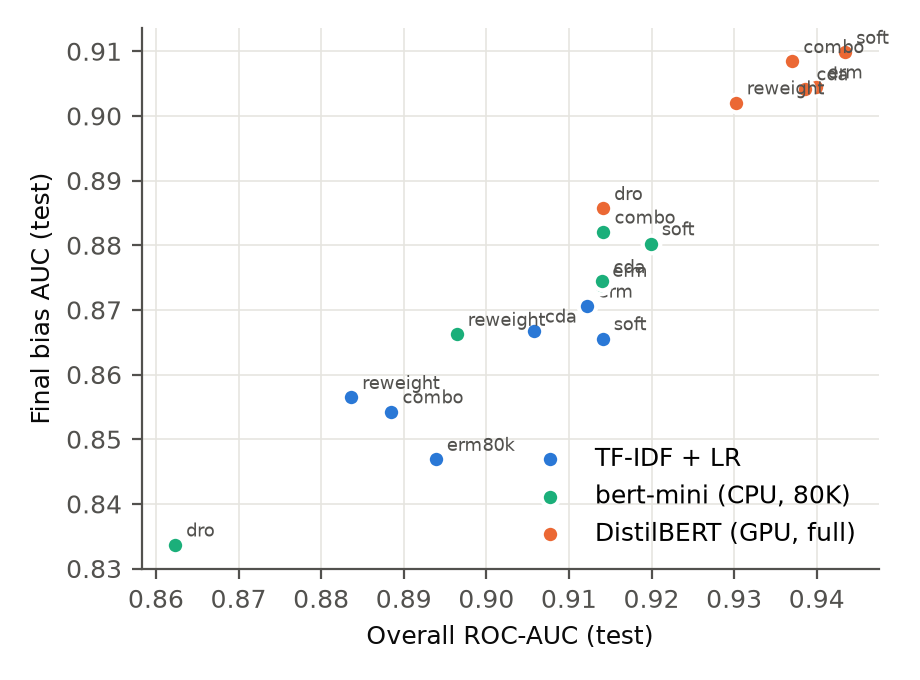
\includegraphics[width=\columnwidth]{../results/fig_tradeoff.png}
\caption{Overall AUC against bias AUC on test for every model (seed 0). Within each family, reweighting and DRO move
down and to the left; soft labels move right, and also up for the two transformers.}\label{fig:tradeoff}
\end{figure}

\paragraph{Templates and deferral.} DistilBERT ERM flags 19\% of the 144 neutral identity sentences (``I'm proud to be
gay.''); reweighting and DRO bring this to 3.5\% and 0\%, and every DistilBERT model except DRO flags all 90 toxic
ones. TF-IDF's neutral sentences about \emph{gay} average $P(\text{toxic}){=}0.70$ (Figure~\ref{fig:templates}).
After temperature scaling, ERM and soft-label DistilBERT are well calibrated (ECE \BertDistilErmEceCal{} and
\BertDistilSoftEceCal{}), and deciding only the 80\% of comments furthest from the threshold cuts the error rate from
0.083 to \BertDistilErmErrAtEightycov{} and \BertDistilSoftErrAtEightycov{} (Figure~\ref{fig:rc}). That is what makes
the defer band useful rather than cosmetic.

\section{Error analysis}
\label{sec:errors}
\paragraph{Errors live where raters disagree.} Heuristic tags on every test comment (Table~\ref{tab:tags}) show that
92\% of DistilBERT's false negatives and 56\% of its false positives have a borderline label (30--70\% of raters said
toxic), against 13.5\% of correct predictions, and identity mentions appear in 61\% of errors against 37\% of correct
predictions.

\begin{table}[t]\centering\small
\resizebox{\linewidth}{!}{\begin{tabular}{lrrr}\toprule
Reason (hand-coded) & FP & FN & Total\\\midrule
Harsh but civil disagreement & 27 & 24 & 51\\
Implicit or coded hostility & 0 & 30 & 30\\
Identity mention, not hostile & 28 & 0 & 28\\
Gold label looks wrong & 11 & 12 & 23\\
Sarcasm or irony & 7 & 13 & 20\\
Genuinely ambiguous & 12 & 6 & 18\\
Quoting or reporting toxicity & 8 & 9 & 17\\
Rude words, not aimed at anyone & 7 & 1 & 8\\
Other: disguised insult or truncation & 0 & 5 & 5\\
Total & 100 & 100 & 200\\
\bottomrule\end{tabular}}
\caption{Main reason for each of 200 test errors of the best model (100 false positives and 100 false negatives, sampled at random), labelled by hand by the author. One label per error.}\label{tab:hand}
\end{table}
\paragraph{Hand coding: why the errors happen.} To check the tags, I took a random sample of 100 false positives and
100 false negatives of the best model and labelled each by hand with the single reason that best explains it, using
categories fixed before coding (Table~\ref{tab:hand}; each count is also a percentage, with a 95\% interval of at most
$\pm$10 points). The two error types have different causes. The largest false-positive group is non-hostile identity
mentions (\HandFPIdentity{}), the failure the mitigations target, and no false negative falls in it. The largest
false-negative group is implicit or coded hostility (\HandFNImplicit{}): stereotypes and dehumanising remarks without
insult words, followed by sarcasm (\HandFNSarcasm{}). Harsh but civil disagreement accounts for \HandFPCivil{} false
positives and \HandFNCivil{} false negatives, so the model and the raters draw the line between criticism and
incivility in different places, in both directions. I judged the gold label wrong in \HandGoldWrong{} errors and could
not decide in \HandAmbiguous{} more; the mislabelled false positives include a slur that 44\% of its 70 raters called
toxic and a comment implying gay men are predators that none of its four raters did. The last \HandOther{} false
negatives are insults the model cannot read: disguised or abbreviated profanity (``fcking'', ``\#\$\%\#ing'',
``POS''), a misspelling (``maroon''), and a slur past the 128-wordpiece cut.

The heuristic tags overstate identity and miss sarcasm. The identity tag fires on \HandIdTagFP{} sampled false
positives, but by hand the identity mention was the cause in only \HandFPIdentity{}; the quote tag catches
\HandQuoteTag{} quoting errors but also fires on \HandQuoteTagElse{} others; and the sarcasm tag catches only
\HandSarcTag{} sarcastic errors.

\paragraph{Confident false positives and attribution.} The most confident identity ``false positives'' are often
label noise: ``You are a NASTY WOMAN'' was called toxic by 32\% of 65 raters. For ERM the top integrated-gradients
word in these comments is usually an insult; an identity term is the top word in only \IGTopErm{} of the 150 most
confident identity-mentioning false positives (top three: \IGTopThreeErm{}). For the soft-label model these rise to
\IGTopBest{} and \IGTopThreeBest{}. A plausible explanation is that soft targets reproduce the raters' own partial
sensitivity to identity mentions: \BenignIdRater{} of benign training comments that mention an identity have at least
one rater calling them toxic, against \BenignNoIdRater{} of those that mention none (mean toxicity fraction
\BenignIdFrac{} vs.\ \BenignNoIdFrac{}). A thresholded label discards that signal; a soft label keeps it. Testing the
explanation directly needs per-rater labels.

\begin{table}[t]\centering\small\setlength\tabcolsep{3pt}
\resizebox{\linewidth}{!}{\begin{tabular}{lrrrrrr}\toprule
& \multicolumn{3}{c}{False positives} & \multicolumn{3}{c}{False negatives}\\
DistilBERT & fixed & new & total & fixed & new & total\\\midrule
ERM & & & 6,666 & & & 4,399\\
+ CDA & 1,647 & 1,226 & 6,245 & 509 & 779 & 4,669\\
+ reweight & 1,960 & 1,781 & 6,487 & 562 & 1,197 & 5,034\\
+ group DRO & 2,945 & 3,660 & 7,381 & 808 & 2,291 & 5,882\\
+ soft labels & 945 & 1,494 & 7,215 & 687 & 369 & 4,081\\
+ combo & 1,586 & 2,682 & 7,762 & 894 & 823 & 4,328\\
\bottomrule\end{tabular}}
\caption{Test errors of each DistilBERT mitigation against ERM (seed 0, each model at its own validation threshold). \emph{fixed}: ERM errors the mitigation gets right; \emph{new}: errors ERM did not make.}\label{tab:fixed}
\end{table}
\paragraph{Every mitigation trades errors.} Against ERM, soft labels fix \FPFixed{} false positives and \FNFixed{}
false negatives but introduce \FPIntro{} and \FNIntro{} new ones (Table~\ref{tab:fixed}). Every mitigation changes
thousands of individual decisions, even where the totals barely move. Reweighting and group DRO introduce the most new
false negatives, and DRO ends with more false positives than ERM overall: it closes the gap without reducing false
alarms. Soft labels and combo are the only mitigations that miss fewer toxic comments than ERM.

\section{The Fair-Mod workbench}
\label{sec:system}
The Gradio app \citep{abid2019gradio} has three tabs. \emph{Moderate} takes typed text or a comment from a queue that
mixes curated hard cases with real test comments chosen by rule (benign identity mentions ERM flags, likely label
noise, missed toxic comments, 50/50 rater splits). For the selected model it shows the calibrated probability against
the model's threshold, a flag/allow/defer decision from a moderator-set band, subtype probabilities, word
attributions, an identity-swap table with the decision for each swap, and, for queue comments, how the raters split.
Further tabs show per-identity test results and the tool's limitations. Everything is computed live.

\section{Discussion}
\paragraph{What the results support.} (1) A stronger pretrained encoder trained on more data reduces identity-related
ranking errors more than any mitigation applied to a weaker model. (2) Soft labels improve ranking quality without lowering
AUC anywhere: higher AUC and worst-group accuracy in all three families, and higher bias AUC for both transformers,
stable across DistilBERT seeds. (3) The FPR gap can be closed, but only by mitigations that raise false negatives on
the same groups and degrade calibration; which of the two errors matters more is a policy choice, not a modelling
result. (4) CDA makes models invariant to the swaps they were trained on and little else.

\paragraph{What they do not support, and limitations.} The audit covers \emph{mentions} of eight coarse groups, not
authors, and says nothing about dialect-based bias \citep{sap2019risk}. Bias AUC differences between DistilBERT
mitigations are small (0.887--0.909) even where they exceed seed noise. The 19\% template flag rate comes from 144
hand-written sentences, so it shows a problem rather than a deployment rate. ``Correct'' means agreeing with a
majority of usually four raters. The swap lexicon also fires on non-identity uses (``black hole'' becomes ``white hole''); the hand coding
has a single coder (the author), so there is no inter-annotator agreement; bert-mini rests on one seed; and
calibration is fit on the same distribution it is tested on.

\paragraph{Next steps.} (1) Test the soft-label hypothesis with per-rater labels, for example by holding out the rater
votes of identity-mentioning comments. (2) Guide CDA with named entity recognition, which tags mentions of nationalities
and religious or political groups, so that only terms referring to people are swapped (no ``white hole''), and add
held-out identities to training. (3) Make the threshold group-aware or add a reject-option rule, which could close the FPR gap without
retraining. (4) Normalise disguised profanity and score long comments in windows, since both explain missed toxic
comments in the hand-coded sample. (5) Evaluate transfer to a second dataset.

\section{Ethics}
The data is public, CC0, and released without user ids; quotes are short and not traceable to authors, and the app
and paper carry content warnings. ``Toxicity'' encodes a particular rater pool's norms, which the model inherits. The
tool is decision support with a defer option, because a ``debiased'' classifier could give automated removal false
legitimacy.

\section{Generative AI disclosure}
I used Claude Opus 5.5 to generate initial implementations for multiple scripts throughout my pipeline and to toubleshoot errors in them as well as hunt for bugs and fix them. I made sure that I understood every line of generated code and have heavily revised the code manually to match my dataset. I frequently tested generated code manually to ensure that it worked as intended and never blindly trusted generated code. Claude was also used to design my slides. However, all content within the slides was generated by me manually and I told Claude exactly what to put on each slide and with what format. Claude also generated all Latex code I used. I know how to use latex myself and I was the one that instructed claude to build the pdf using latex. However, I am not fast at writing latex so I instead wrote the entirety of the report on a google doc which I then gave to claude for the purposes of transforming it into latex code. When it comes to prose, claude was used for syntactical, vocabulary, grammar, and spelling corrections, after my report was already complete. The part of my report referencing Named Entity Recognition models was suggested to me by my TA as feedback during the oral defense. 

\section*{Reproducibility}
{\raggedright Code: \url{https://github.com/taxpet06/fair-mod}; data: the CC0 WILDS mirror in Section~\ref{sec:data}.
The README gives setup, pinned requirements, and run times. After \texttt{pip install -r requirements.txt} and
\texttt{./download\_data.sh}, the analysis runs as \texttt{tfidf.py}, \texttt{bert.py} per variant, \texttt{evaluate.py},
\texttt{errors.py}, and \texttt{report/build\_tables.py}; \texttt{app.py} starts the workbench. Seeds are fixed.
Tables and macro numbers are generated from \texttt{results/}; other numbers were typed from the same CSVs, except the
proposal's exploration figures and the laptop throughputs.\par}


\bibliography{refs}

\clearpage
\appendix
\section*{Supplementary material}
\section{Additional results}
\label{app:more}
Counterfactual probes (Table~\ref{tab:cf}), per-identity metrics (Table~\ref{tab:identity}), heuristic error tags
(Table~\ref{tab:tags}), risk-coverage (Figure~\ref{fig:rc}), and per-identity FPR and template scores
(Figure~\ref{fig:templates}).

\begin{table}[t]\centering\small\setlength\tabcolsep{3pt}
\resizebox{\linewidth}{!}{\begin{tabular}{lccccc}\toprule
& \multicolumn{3}{c}{Template spread $\downarrow$} & Real & Neutral\\
Model & all & seen & held-out & $|\Delta p|$ $\downarrow$ & flagged $\downarrow$\\\midrule
B2 ERM & 0.133 & 0.148 & 0.020 & 0.041 & 20\%\\
\quad ERM, 80K subsample & 0.101 & 0.114 & 0.029 & 0.037 & 19\%\\
\quad + reweight & 0.155 & 0.173 & 0.080 & 0.047 & 12\%\\
\quad + CDA & 0.135 & 0.109 & 0.031 & 0.011 & 27\%\\
\quad + soft labels & 0.108 & 0.118 & 0.026 & 0.036 & 15\%\\
\quad + combo & 0.108 & 0.094 & 0.041 & 0.009 & 19\%\\
\midrule
bert-mini ERM (80K, CPU) & 0.123 & 0.125 & 0.114 & 0.035 & 26\%\\
\quad + reweight & 0.125 & 0.135 & 0.096 & 0.032 & 8\%\\
\quad + CDA & 0.088 & 0.086 & 0.072 & 0.015 & 27\%\\
\quad + group DRO & 0.101 & 0.101 & 0.093 & 0.030 & 1\%\\
\quad + soft labels & 0.080 & 0.079 & 0.079 & 0.027 & 15\%\\
\quad + combo & 0.096 & 0.100 & 0.073 & 0.013 & 11\%\\
\midrule
B3 DistilBERT ERM & 0.114 & 0.122 & 0.088 & 0.038 & 19\%\\
\quad + reweight & 0.109 & 0.116 & 0.090 & 0.037 & 3\%\\
\quad + CDA & 0.101 & 0.094 & 0.094 & 0.012 & 21\%\\
\quad + group DRO & 0.126 & 0.123 & 0.121 & 0.033 & 0\%\\
\quad + soft labels & 0.081 & 0.095 & 0.036 & 0.033 & 16\%\\
\quad + combo & 0.112 & 0.109 & 0.103 & 0.009 & 12\%\\
\bottomrule\end{tabular}}
\caption{Counterfactual probes. \emph{Template spread}: mean absolute deviation of $P(\text{toxic})$ from the template mean across 18 identity terms (8 neutral and 5 toxic templates), split into terms in the CDA lexicon (\emph{seen}) and 5 held-out terms (sikh, queer, arab, mexican, african american). \emph{Real}: mean $|p(\text{swap})-p(\text{original})|$ over in-category swaps of 2{,}000 test comments. \emph{Neutral flagged}: share of the 144 neutral template sentences above the model's threshold.}\label{tab:cf}
\end{table}
\begin{table}[t]\centering\small\setlength\tabcolsep{3pt}
\resizebox{\linewidth}{!}{\begin{tabular}{lcccccc}\toprule
& \multicolumn{3}{c}{bert ERM} & \multicolumn{3}{c}{best}\\
Tag & FP & FN & ok & FP & FN & ok\\\midrule
identity mention & 62\% & 61\% & 37\% & 60\% & 62\% & 37\%\\
profanity & 5\% & 4\% & 2\% & 5\% & 4\% & 2\%\\
insult word & 15\% & 9\% & 4\% & 14\% & 9\% & 4\%\\
quote or reported & 30\% & 36\% & 30\% & 30\% & 37\% & 30\%\\
sarcasm marker & 4\% & 5\% & 4\% & 4\% & 5\% & 4\%\\
borderline label & 56\% & 92\% & 14\% & 56\% & 92\% & 14\%\\
few raters ($<$6) & 24\% & 2\% & 66\% & 23\% & 2\% & 66\%\\
$n$ & 6,666 & 4,399 & 121,542 & 7,215 & 4,081 & 121,311\\
\bottomrule\end{tabular}}
\caption{Share of test comments carrying each heuristic tag, by outcome. \emph{borderline label}: 30--70\% of raters said toxic.}\label{tab:tags}
\end{table}
\begin{table*}[t]\centering\small
\resizebox{\linewidth}{!}{\begin{tabular}{lrrccccccccc}\toprule
& & & \multicolumn{3}{c}{BPSN AUC $\uparrow$} & \multicolumn{3}{c}{FPR $\downarrow$} & \multicolumn{3}{c}{FNR $\downarrow$}\\
Identity & $n$ & toxic & TF-IDF & ERM & best & TF-IDF & ERM & best & TF-IDF & ERM & best\\\midrule
LGBTQ & 4,390 & 27\% & 0.783 & 0.829 & 0.838 & 0.200 & 0.204 & 0.204 & 0.352 & 0.273 & 0.272\\
black & 4,826 & 31\% & 0.721 & 0.798 & 0.821 & 0.277 & 0.242 & 0.234 & 0.287 & 0.247 & 0.247\\
christian & 13,277 & 9\% & 0.925 & 0.947 & 0.947 & 0.048 & 0.046 & 0.050 & 0.491 & 0.386 & 0.359\\
female & 16,309 & 14\% & 0.886 & 0.923 & 0.929 & 0.072 & 0.071 & 0.074 & 0.403 & 0.328 & 0.315\\
male & 14,185 & 15\% & 0.873 & 0.913 & 0.919 & 0.085 & 0.086 & 0.091 & 0.375 & 0.308 & 0.290\\
muslim & 6,861 & 23\% & 0.798 & 0.861 & 0.870 & 0.163 & 0.141 & 0.145 & 0.388 & 0.332 & 0.327\\
other religions & 3,454 & 15\% & 0.863 & 0.908 & 0.910 & 0.101 & 0.084 & 0.095 & 0.395 & 0.386 & 0.353\\
white & 7,828 & 28\% & 0.733 & 0.812 & 0.824 & 0.250 & 0.208 & 0.220 & 0.284 & 0.274 & 0.261\\
\bottomrule\end{tabular}}
\caption{Per-identity test metrics for TF-IDF ERM, DistilBERT ERM, and the best mitigated DistilBERT model by validation bias AUC (\texttt{bert\_distil\_soft}). BPSN AUC is low when non-toxic comments that mention the group score above toxic comments that don't.}\label{tab:identity}
\end{table*}
\begin{figure}[t]\centering
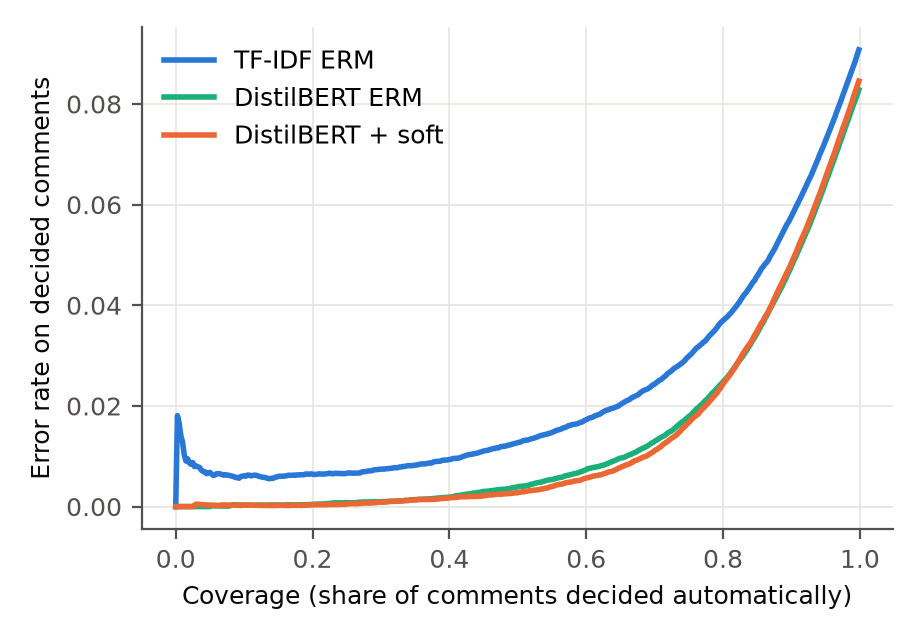
\includegraphics[width=\columnwidth]{../results/fig_risk_coverage.png}
\caption{Risk-coverage on test: error rate among the comments decided automatically, when the least confident are
deferred first. Confidence is the logit distance from each model's validation threshold.}\label{fig:rc}
\end{figure}
\begin{figure*}[t]\centering
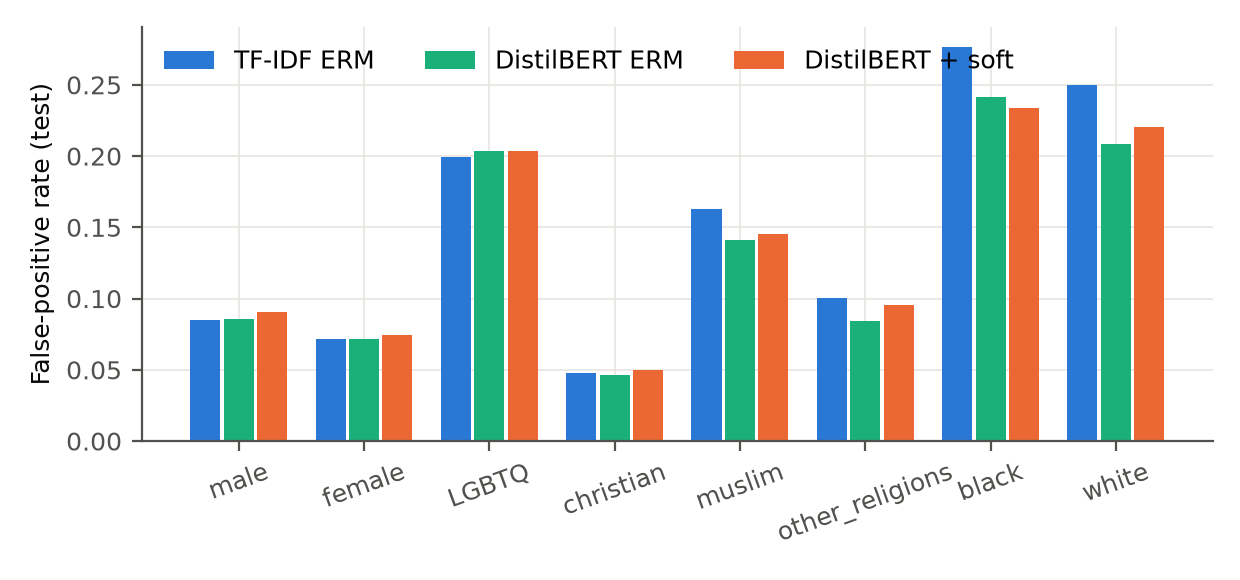
\includegraphics[width=0.49\textwidth]{../results/fig_fpr_by_identity.png}\hfill
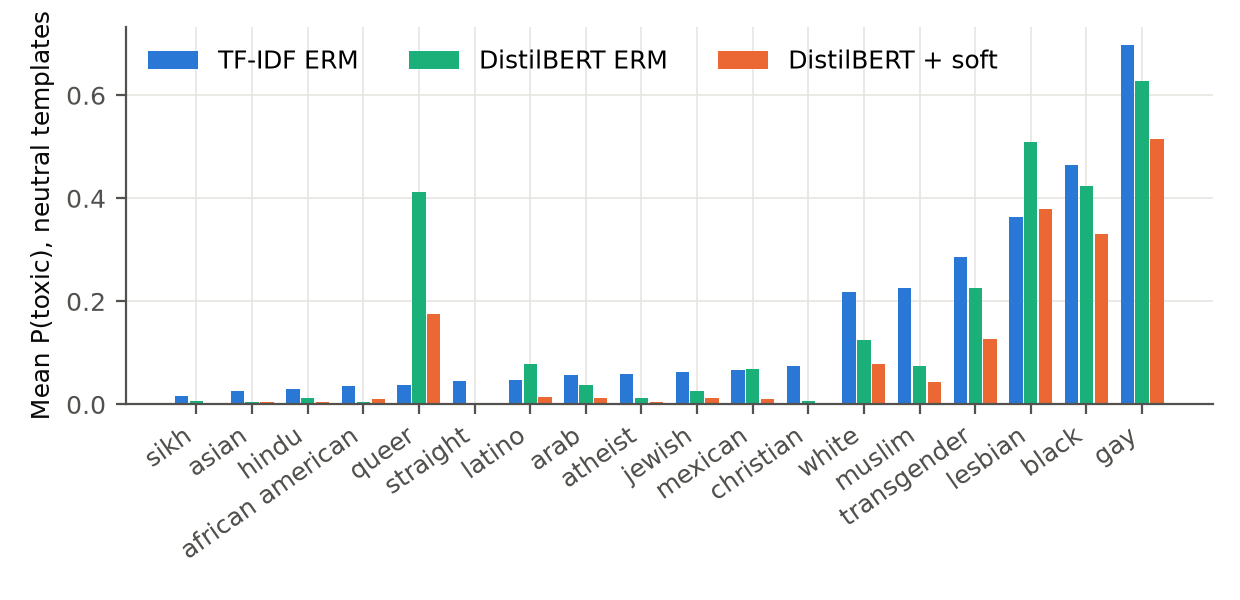
\includegraphics[width=0.49\textwidth]{../results/fig_templates.png}
\caption{Left: test FPR by identity. Right: mean $P(\text{toxic})$ on neutral template sentences by identity term,
sorted by TF-IDF ERM. The ERM models' worst FPRs are on \emph{black}, \emph{white}, \emph{LGBTQ}, and
\emph{muslim}.}\label{fig:templates}
\end{figure*}

\onecolumn
\section{Changes from the proposal}
\label{app:changes}
\begin{center}\small
\begin{tabular}{p{0.24\textwidth}p{0.30\textwidth}p{0.38\textwidth}}\toprule
Proposal & Final & Why \\\midrule
Training on university GPU servers & DistilBERT on the Dartmouth Discovery cluster (free-tier \texttt{gpu\_preempt}: H200, A5000/A5500, RTX 2080 Ti); bert-mini on a 12-core laptop CPU & As proposed for B3. Jobs stream code and data over \texttt{srun} stdin/stdout because GPU nodes cannot read home storage. The CPU runs are kept as a compute-constrained comparison (bert-mini ${\sim}150$, bert-small ${\sim}18$, DistilBERT ${\sim}7$ train examples/s on the laptop). \\
DistilBERT or RoBERTa-base (B3) & DistilBERT, full 267K training split, 1 epoch; plus bert-mini on an 80K subsample & DistilBERT matches the proposal. RoBERTa-base was not run. A same-subsample TF-IDF run (\texttt{erm80k}) separates data size from model family. \\
Three seeds for neural models & Three seeds for every DistilBERT variant; one for bert-mini & DistilBERT seeds are cheap on the cluster. bert-mini runs took ${\sim}40$ CPU-minutes each, so its comparisons rest on bootstrap CIs, which cover test sampling only. \\
Soft labels from the 1.8M Hugging Face pool & Soft labels joined by comment id from the WILDS raw file & Same annotator fractions without the cross-release leakage risk (90.5\% text overlap). The 1.8M pool is unused. \\
Truncate at 256 subword tokens & 128 wordpieces for every transformer & Fixed for the CPU bert-mini runs and kept for DistilBERT so the families share one recipe. It truncates \TokOverOneTwoEight{} of test comments, against \TokOverTwoFiveSix{} at 256; one hand-coded missed slur sits past the cut (Section~\ref{sec:errors}). \\
Captum for integrated gradients & 20-line hand-written IG with a completeness self-check & Avoids a dependency; the completeness axiom is checked numerically. \\
Group DRO on both model families & transformers only & DRO needs a per-batch loss loop; sklearn's logistic regression has none. \\
200 hand-coded errors & 200 hand-coded errors of the best model, 100 FP and 100 FN (\texttt{results/}\allowbreak\texttt{errors\_hand\_coded.csv}), plus heuristic tags on all errors & As proposed. The hand labels are the author's own; the automated tags extend coverage to every error and are checked against the hand labels (Section~\ref{sec:errors}). \\
\bottomrule\end{tabular}
\end{center}

\section{Settings}
\label{app:settings}
\begin{center}\small
\begin{tabular}{lp{0.74\textwidth}}\toprule
TF-IDF & word 1--2 grams, min\_df 3, 300{,}000 features, sublinear tf; vectoriser fit once on the training split \\
Logistic regression & L2, $C{=}4$, liblinear, max\_iter 300 \\
DistilBERT & \texttt{distilbert-base-uncased}, 7 sigmoid heads, mean BCE, lr $5{\times}10^{-5}$, bf16 autocast where supported, full training split \\
bert-mini & \texttt{prajjwal1/bert-mini}, tokenizer \texttt{bert-base-uncased}, same heads, lr $10^{-4}$, CPU \\
Optimisation & AdamW, weight decay 0.01, batch 32, 1 epoch, 6\% linear warm-up then linear decay, grad-norm clip 1.0 \\
Sequence length & 128 wordpieces, dynamic padding, length-bucketed shuffled batches \\
Training data & DistilBERT: all 267{,}112 training comments. bert-mini: 80{,}000 sampled with seed 0 (same sample for every variant). CDA adds copies \\
Reweighting & inverse frequency of 18 groups, normalised to mean 1, clipped at 10 \\
Group DRO & online exponentiated gradient over 18 groups, $\eta{=}0.01$ \\
Calibration & one temperature on the toxicity logit, grid over $[0.25, 4]$, minimum validation NLL \\
Threshold & validation-F1-optimal over $\{0.05, 0.06, \dots, 0.95\}$ \\
IG & [PAD]-embedding baseline, special tokens fixed, 48 steps (32 in the error analysis) \\
Bootstrap & 50 test-set resamples, percentile 95\% interval \\
Seeds & data subsample fixed at 0; training seed 0 (all models) and 1, 2 (DistilBERT) \\
\bottomrule\end{tabular}
\end{center}

\end{document}
